%% ma: L11-B15-0083
%% lop: 11
%% chuong: 5
%% bai: 15
%% dang: 11.15.9
%% loai: TLN
%% muc: VD
%% dap_an: "13,7"
%% nguon: "tai-lieu-hoc-tap-mon-toan-lop-11-theo-chuong-trinh-giao-duc-pho-thong-2018.pdf (Lớp Toán Thầy Duy, Phạm Lê Duy, THPT Chu Văn An), Chương 3 Bài 1, Phần 3, Câu 5 (tr.340)"
%% kien_thuc: "Lớp 11 Bài 15; Bài 7 (cấp số nhân)"
%% trang_thai: cho-duyet
%% ly_do: "Dạng mới đề xuất (11.15.x), chờ giáo viên duyệt dạng; tài liệu gốc không có lời giải mẫu, đáp án do kho tự giải và kiểm bằng sympy."
%% ghi_chu: "Hình TikZ do kho dựng (5 hình vuông đầu), thay hình gốc."
\begin{ex}
Cho hình vuông $ABCD$ có cạnh bằng $1$. Nối các trung điểm của bốn cạnh hình vuông $ABCD$, ta được hình vuông thứ hai. Tiếp tục nối các trung điểm của bốn cạnh hình vuông thứ hai, ta được hình vuông thứ ba. Tiếp tục như thế ta nhận được một dãy các hình vuông. Tìm tổng chu vi của dãy các hình vuông đó (kết quả làm tròn đến hàng phần mười).
\begin{center}
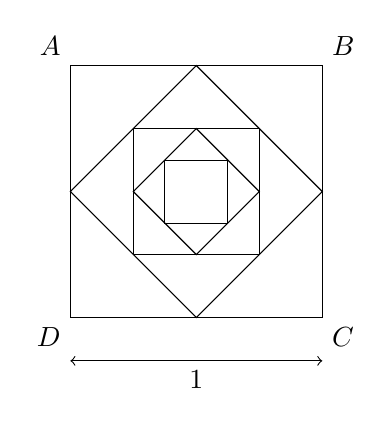
\begin{tikzpicture}
\draw (0.0000,0.0000) -- (3.2000,0.0000) -- (3.2000,3.2000) -- (0.0000,3.2000) -- cycle;
\draw (1.6000,0.0000) -- (3.2000,1.6000) -- (1.6000,3.2000) -- (0.0000,1.6000) -- cycle;
\draw (2.4000,0.8000) -- (2.4000,2.4000) -- (0.8000,2.4000) -- (0.8000,0.8000) -- cycle;
\draw (2.4000,1.6000) -- (1.6000,2.4000) -- (0.8000,1.6000) -- (1.6000,0.8000) -- cycle;
\draw (2.0000,2.0000) -- (1.2000,2.0000) -- (1.2000,1.2000) -- (2.0000,1.2000) -- cycle;
\node[above left] at (0,3.2) {$A$}; \node[above right] at (3.2,3.2) {$B$};
\node[below right] at (3.2,0) {$C$}; \node[below left] at (0,0) {$D$};
\draw[<->] (0,-0.55)--(3.2,-0.55) node[midway,below] {$1$};
\end{tikzpicture}
\end{center}
\shortans{13,7}
\loigiai{\sloppy Cạnh hình vuông sau bằng $\dfrac{\sqrt2}2$ lần cạnh hình vuông trước, nên chu vi lập thành cấp số nhân lùi vô hạn có $u_1=4$, $q=\dfrac{\sqrt2}2$. Tổng chu vi $=\dfrac4{1-\frac{\sqrt2}2}=8+4\sqrt2\approx13{,}7$.}
\end{ex}
